\section{Metodologia dos experimentos}
\label{sec:dtw-metodology}

A metodologia utilizada neste modelo pode ser dividida em duas partes: (1) o processo da indexação do banco de dados de referência e; (2) como funciona o processo de identificação das janelas do banco de dados e apontamento das previsões.

\subsection{Indexação do banco de dados de referência}
\label{subsec:database_dtw}

Como mencionado na \subsecref{subsec:indexation_and_identification}, o banco de dados de referência para esse modelo respeita um conjunto de três regras. Portanto, para os nossos experimentos, precisamos organizar as sequências de referência respeitando-as.

Uma forma de visualizar como os dados podem ser estruturados é transformando as sessões de uma música em uma espécie de máquina de estados, como a ilustrada na \figref{fig:miab_state_machine} para a música \textit{Message In A Bottle} para a trilha da guitarra elétrica de base. Como exemplo, em um corte da partitura da música, demonstrada na \figref{fig:miab_sheet_music}, é possível visualizar como esses estados estão organizados dentro dos compassos.

\begin{figure}[htbp]
    \centering
    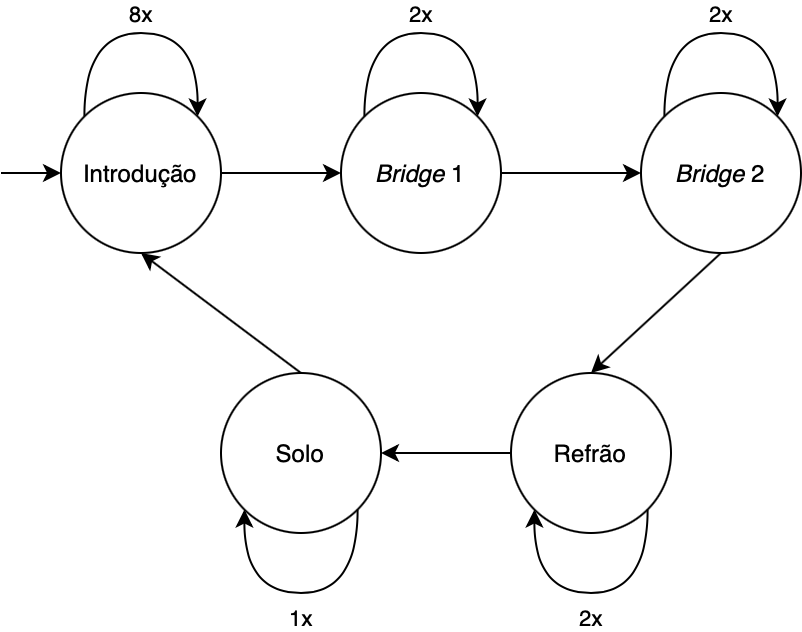
\includegraphics[width=0.75\textwidth]{images/MIAB state machine.png}
    \caption{Máquina de estados para a trilha da guitarra elétrica de base da música \textit{Message In A Bottle} (\textit{The Police}, 1979).}
    \label{fig:miab_state_machine}
\end{figure}

\begin{figure}[htbp]
    \centering
    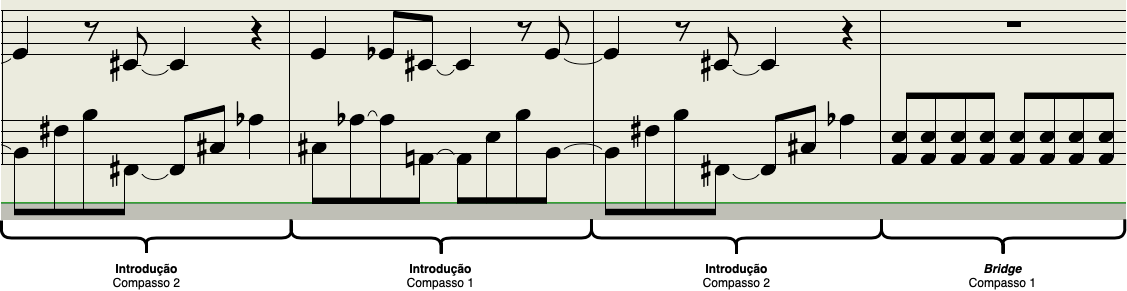
\includegraphics[width=1\textwidth]{images/dtw-real division.png}
    \caption{Relação dos estados da \figref{fig:miab_state_machine} com compassos em um trecho da partitura da trilha da guitarra elétrica da música \textit{Message In A Bottle} (\textit{The Police}, 1979).}
    \label{fig:miab_sheet_music}
\end{figure}

No entanto, é notável que alguns estados podem transitar para mais de um estado - por exemplo, a introdução pode transitar entre si mesma em \textit{loop} ou para o \textit{bridge}. Tal característica quebra a Regra 3, pois, caso o estado identificado fosse a introdução, não seria possível saber qual seria o próximo estado e duas previsões seriam entregues, causando ambiguidade.

Para lidar com isso, podemos reorganizar tal máquina apresentando estados de transição. Dessa forma, quando uma transição fosse identificada, apenas uma previsão seria gerada, como ilustrado na \figref{fig:miab_adapted_state_machine}. Note, entretanto, que nenhum dos estados ``aponta'' para um estado de transição. Isso significa os cortes de áudio que representam essas transições nunca será apontado como uma previsão, efetivamente perdendo essa informação na transmissão do músico remoto.

\begin{figure}[htbp]
    \centering
    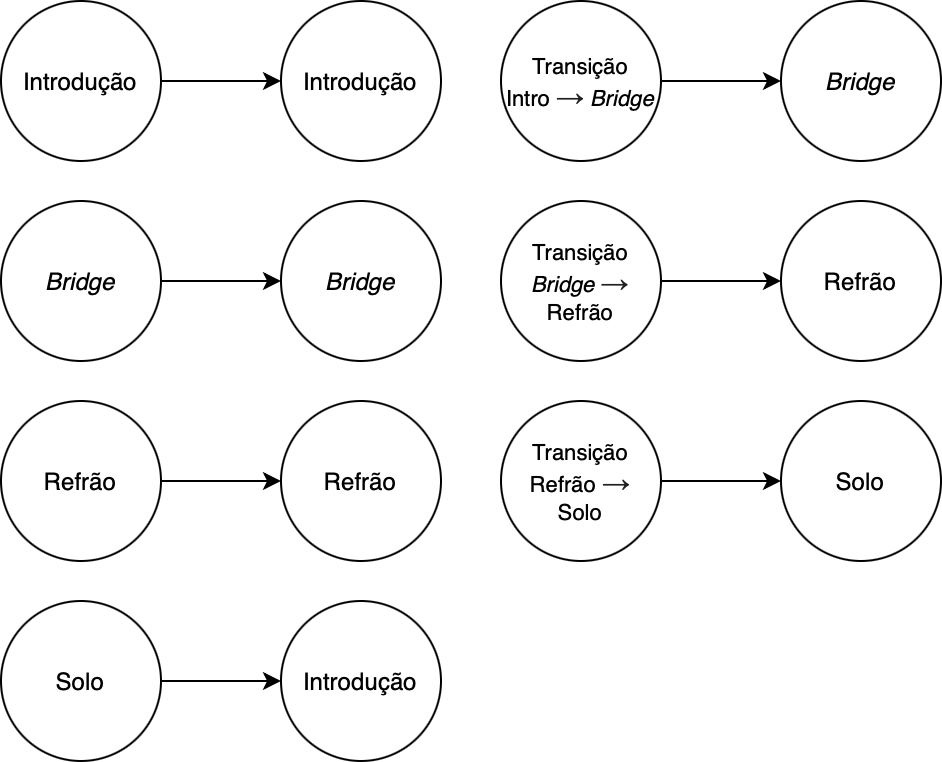
\includegraphics[width=0.75\textwidth]{images/MIAB adapted state machine.png}
    \caption{Máquina de estados adaptada para a trilha da guitarra elétrica da música \textit{Message In A Bottle} (\textit{The Police}, 1979).}
    \label{fig:miab_adapted_state_machine}
\end{figure}

Ao dividir as janelas de referência, portanto, é necessário escolher cortes onde seja possível identificar as transições. Se usarmos a divisão de compassos que a partitura original oferece, não seria possível identificar quando termina um \textit{loop} e quando a próxima sessão inicia. Portanto, cada sequência da música necessita possuir um pequeno corte à sua frente. A forma que fazemos isso é movendo cada janela em meio compasso para frente no tempo, como ilustrado na \figref{fig:miab_windowed_sheet_music} - dessa forma, dois compassos estarão presentes em uma mesma janela e, portanto, é possível identificar transições.

\begin{figure}[htbp]
    \centering
    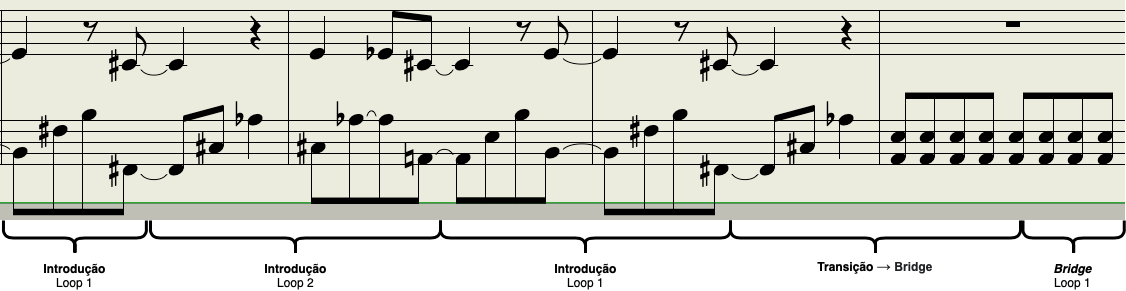
\includegraphics[width=1\textwidth]{images/dtw-window division.png}
    \caption{Relação dos estados da \figref{fig:miab_adapted_state_machine} com um corte da partitura original da trilha da guitarra elétrica da música \textit{Message In A Bottle} (\textit{The Police}, 1979). Movendo as janelas meio compasso à frente, é possível criar janelas de transição.}
    \label{fig:miab_windowed_sheet_music}
\end{figure}

Em nossos experimentos, identificamos e separamos cada estado manualmente, assim como construímos a máquina de estados de referência, semelhante à apresentada na \figref{fig:miab_adapted_state_machine}. Para a música \textit{Message In A Bottle}, utilizamos duas unidades de divisão para experimentação: uma onde cada janela de referência possuía dois compassos de duração (3,158 segundos) e outra onde possuíam um compasso de duração (1,579 segundos).

Também realizamos testes com a introdução da música \textit{Hotel California}, que, diferentemente de \textit{Message In A Bottle}, não possui \textit{loops}. Com isto, não havia necessidade da identificação de janelas de transição, tornando a máquina de estados linear. Para ests música, experimentamos durações de 1, 2 e 3 segundos para cada janela de referência.

\subsection{Processo de identificação das janelas e apontamento das previsões}

Uma vez que possuímos o banco de dados de referência organizado, podemos realizar a identificação para as sequências de entrada, transmitidas pelo músico remoto. Como mencionado na \subsecref{subsec:indexation_and_identification}, utilizamos o algoritmo de alinhamento de séries temporais, o DTW (\textit{Dynamic Time Warping}) \cite{dtw}, especificamente a implementação da biblioteca Librosa \cite{librosa}, em Python.

A função do DTW pode receber diversos argumentos. Para nossos experimentos, utilizamos três deles: (1) uma matriz de \textit{features} da sequência de referência; (2) uma matriz de \textit{features} da sequência de pesquisa e; (3) o booleano $subseq$, que indica se a sequência de pesquisa está contida como subsequência na primeira sequência - em nosso caso, enviamos esse argumento como $True$.

Note que os dois primeiros argumentos requerem matrizes de \textit{features} das sequências de áudio. Para a primeira matriz, juntamos todos os arquivos de áudio da base de dados de referência em um único, e retiramos seu chromagrama \cite{chromagram}, também implementado pela Librosa, que retorna uma tabela das notas musicais mais presentes na sequência em função do tempo. Para a segunda matriz, utilizamos a mesma função para a sequência de pesquisa, simulando o áudio transmitido pelo músico remoto.

Já que configuramos como ``verdadeiro'' o valor o booleano $subseq$, o algoritmo já nos dirá que corte do banco de dados de referência a nossa janela de pesquisa é mais semelhante. Observe, por exemplo, a \figref{fig:dtw_hotel_california} para a música \textit{Hotel California} - ao separar em janelas de 3 segundos, o DTW nos entregará os pontos, em segundos, sob a qual essa sequência de pesquisa se encaixa na base de referência. Com esses valores, é possível identificar qual janela de referência foi identificada - na imagem, foi a \#1. No caso da música \textit{Hotel California}, como sua máquina de estados é linear na introdução, a previsão seria a janela \#2.

\begin{figure}[htbp]
    \centering
    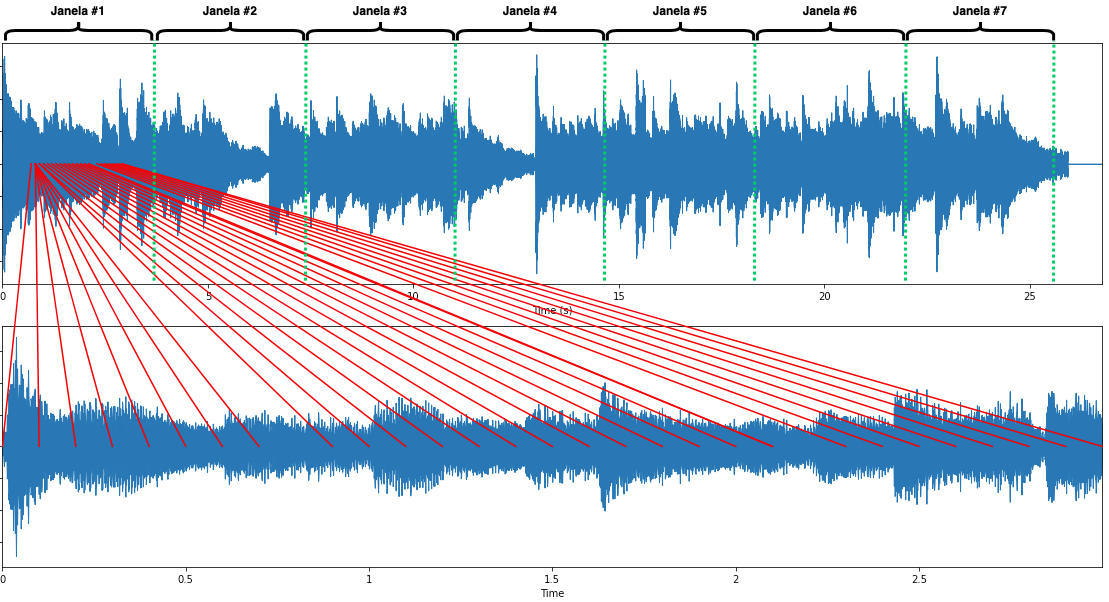
\includegraphics[width=1\textwidth]{images/dtw hotel California.png}
    \caption{Execução do algoritmo DTW para a primeira janela de três segundos para a música Hotel California. Acima, a base de dados de referência; abaixo, a sequência de pesquisa, transmitida pelo músico remoto em nossa simulação; em vermelho, as linhas representam o alinhamento da série temporal entregues pelo algoritmo.}
    \label{fig:dtw_hotel_california}
\end{figure}

Para calcular a taxa de sucesso das identificações, montamos um arquivo de referência que diz, para cada sequência de entrada, qual deve ser a janela correta na base de dados - caso haja correspondência, consideramos a identificação como correta. Para as previsões, utilizamos o mesmo conceito, porém, subtraindo as instâncias onde janelas de transição foram identificadas, já que assumimos a impossibilidade de prevê-las.

Para a medição de performance, consideramos o tempo levado para identificar a janela com DTW e de reproduzir a previsão.

Uma vez que todas as janelas passaram pelo processo completo, juntamos todas as sequências de previsões apontadas em um arquivo WAV para análise \footnote{As previsões geradas podem ser encontradas em \url{https://cutt.ly/2vNvRfy}.}.